\documentclass{report}

% Basic packages and settings
\usepackage{xcolor}
\usepackage[normalem]{ulem}
\usepackage{indentfirst}
    \setlength{\parindent}{2.5em}
    \setlength{\lineskiplimit}{3pt}
    \setlength{\lineskip}{3pt}
\usepackage{geometry}
    \geometry{top = 0.8in, bottom = 1in}
\usepackage{graphicx}
    \graphicspath{{./mpl-image/}}
\usepackage[section]{placeins}
\usepackage{array}

% Contents, Appendix, and Chapter format
\renewcommand{\contentsname}{Table of Contents}

% Bibliography & Index
\usepackage[numbib]{tocbibind}
\usepackage[square,super,sort&compress]{natbib}

% My newcommand & newenvironment
\newcommand{\pkg}[1]{\texttt{#1}}
    \newcommand{\Py}{\pkg{Python}}
    \newcommand{\NumPy}{\pkg{NumPy}}
    \newcommand{\SciPy}{\pkg{SciPy}}
\newcommand{\mpl}{\texttt{Matplotlib}}
\newcommand{\Emph}[1]{\textcolor{cyan!80!white}{{\bfseries #1}}}
\newcommand{\nextblock}{\vspace{2ex}}
\newcommand{\smallquote}[3][0.8ex]{\begin{quote}
    \flushright\emph{#2}\\[#1]
    \ttfamily\rule[0.5ex]{2em}{0.8pt} #3\end{quote}}

% List settings
\usepackage{enumitem}
\setlist[enumerate]
    {font=\bfseries,labelindent=0pt,itemsep=0pt,parsep=0pt,topsep=1ex,partopsep=0pt}
\setlist[itemize]
    {font=\bfseries,itemsep=0pt,parsep=0pt,topsep=1ex,partopsep=0pt}
\setlist[description]
    {font=\bfseries\textbullet\ttfamily~,itemsep=0pt,parsep=0pt,topsep=1ex,partopsep=0pt}

% Code
\usepackage{tcolorbox}
    \tcbuselibrary{listings,skins,breakable}
% Avoid copy line numbers of the listing code
\usepackage{accsupp}
	\newcommand{\emptyaccsupp}[1]{\BeginAccSupp{ActualText={}}#1\EndAccSupp{}}
% Code-only Environment
\newtcblisting{py}{breakable,skin=bicolor,colback=gray!30!white,
    colbacklower=white,colframe=cyan!75!black,listing only, 
    left=6mm,top=2pt,bottom=2pt,
    % listing style
    listing options={language=Python,basicstyle=\small\ttfamily,
    keywordstyle=\color{blue},commentstyle=\color{green!50!black},
    numbers=left,numberstyle=\tiny\color{red!75!black}\emptyaccsupp,
    emptylines=1,escapeinside=``}}
% Inline Python commands
\newtcbox{\python}[1][green]{on line,before upper=\ttfamily,
    arc=0pt,outer arc=0pt,colback=#1!10!white,colframe=#1!50!black,
    boxsep=0pt,left=1pt,right=1pt,top=1pt,bottom=1pt,
    boxrule=0pt,bottomrule=1pt,toprule=1pt}

% Hyperref
\usepackage{hyperref}
    \hypersetup{colorlinks, bookmarksopen = true, bookmarksnumbered = true, pdftitle=Python-matplotlib, pdfauthor=K.L Wu, pdfstartview=FitH}

% Cover of Report
\title{\flushright\framebox{\Huge Simple \mpl} \\[0.4ex]
with basic \NumPy \\[2.5ex]
\ttfamily K.L Wu \\[4ex]
\rmfamily\fontsize{12}{18}\selectfont
Last revision\footnote{Github: \url{https://github.com/wklchris/Note-by-LaTeX/tree/master/python-matplotlib-en}}: \\
\today
}
\author{}
\date{}

\begin{document}

\maketitle

\tableofcontents

\listoffigures

\chapter{Introduction}
\mpl\ is a package of \Py\ (\url{https://www.python.org/}) and it provides strong 2D plotting support. Here are some features of it:
\begin{enumerate}
\item It can be used in both \Emph{interactive} and \Emph{non-interactive} mode.
\item It is allowed to export \Emph{raster} or \Emph{vector} images. Supporting formats include: PNG, JPG, BMP (Raster); EPS, SVG, TIFF, PDF (Vector).
\item Similar syntax with MATLAB, but might have better visualization performance.
\item It's integrated with \LaTeX\ markup.
\end{enumerate}

Visit its main website: \url{http://matplotlib.org/} to find more information and sample images of \mpl .

\section{How to get it?}
You can simply install a distribution of \Py, say, Anaconda (\href{https://www.continuum.io/downloads}{Free download here}), to make sure \mpl\ is installed on your computer. 

If you are an advanced \Py\ user, you can also install \mpl\ package by yourself. Running the setup.py script or downloading unofficial .whl files from \href{http://www.lfd.uci.edu/~gohlke/pythonlibs/#matplotlib}{UC Irvine Unofficial whl \Py\ Downloadpage} and run command line: \texttt{pip install matplotlib.whl} both works.

\section{Dependencies}
You should first install \NumPy\ before getting \mpl .

\NumPy\ is a basic \Py\ module for data works under \Py . It provides high calculation accurancy, many useful predefined math functions, and easier matrices access for \Py\ users. Visit \url{http://www.numpy.org/} for more details.

To check whether you have already had a \NumPy\ installed on your computer, use command line as below:
\begin{verbatim}
... > python
...
>>> import numpy
>>> print(numpy.__version__)
1.11.1
\end{verbatim}

\nextblock This manual is written under Windows operating system and \Py\ 3. You can search for more dependencies if you are a non-Windows users.

\section{Hello, world: the very first example}
Here comes the very beginning of drawing a plot with \mpl :
\begin{py}
import matplotlib.pyplot as plt
plt.plot([0, 2, 3, 1])
plt.show()
\end{py}

And we get a picture like \autoref{fig:interface}:

\begin{figure}[!htb]
  \centering
  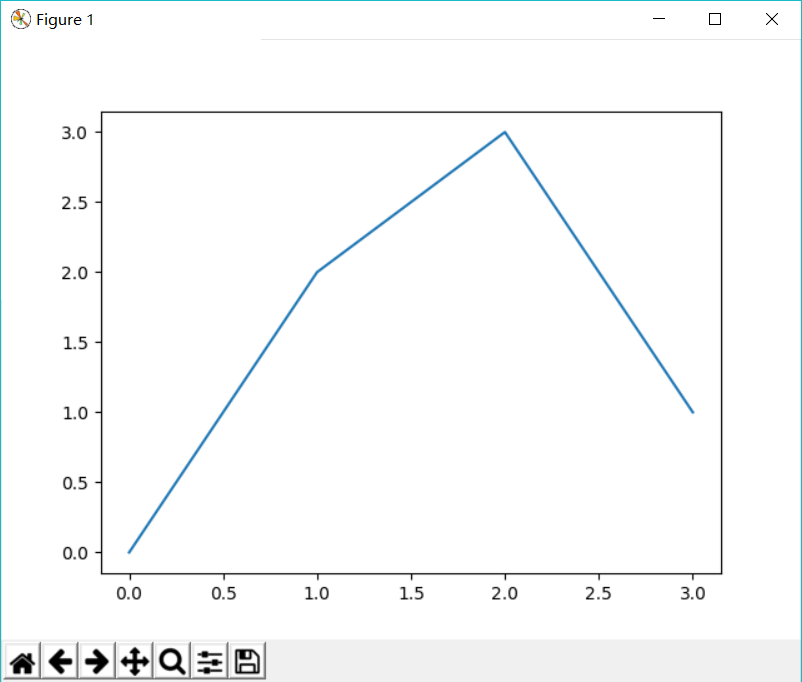
\includegraphics[width=90mm]{Example-Interface.png}
  \caption{The interface of \mpl\ figure window}
  \label{fig:interface}
\end{figure}

We are going to read this example line-by-line.

\subsection{Import \mpl}
Let's focus on the first sentence:
\begin{py}
import matplotlib.pyplot as plt
\end{py}

Usually we won't import the whole \mpl\ package. In this example, we only import the \texttt{pyplot} module of \mpl , which is written as ``\texttt{import matplotlib.pyplot}''. Actually, this module is the most frequently used one. 

Its name is too long for the lazies to type. So use ``\texttt{as plt}'' to let Python know we will use ``\texttt{plt}'' instead of ``\texttt{matplotlib.pyplot}'' below.

NEVER recommand you to behave like below. Please avoid being so greedy and lazy.
\begin{py}
from matplotlib import * # NEVER recommand
\end{py}

\subsection{Simple \texttt{plt} command}
And the second line:
\begin{py}
plt.plot([0, 2, 3, 1])
\end{py}

The command \texttt{plot} provided by \python{plt} (i.e. \texttt{matplotlib.pyplot}) is used to draw a figure. In this example, \mpl\ will first draw points at $(0,0)$, $(1,2)$, $(2,3)$, and $(3,1)$. Then it will connect these points by straight lines.

And maybe it's more clear if you write like this:
\begin{py}
x = [0, 1, 2, 3]
y = [0, 2, 3, 1]
plt.plot(x, y)
\end{py}

\nextblock Users who know how to use \NumPy\ can also do this instead:
\begin{py}
# import numpy as np
x = np.linspace(0, 4, 4)
y = [0, 2, 3, 1]
plt.plot(x, y)
\end{py}

\subsection{Show the figure}
The last line of the example is to show the figure:
\begin{py}
plt.show()
\end{py}

\section{Figure Interface}
If you run those commands, you will get a window like \autoref{fig:interface}. Buttons listed on the bottom of the window are:

\begin{description}[labelindent=.5\parindent]
\item[House:] Reset original view of figure.
\item[Arrows:] Redo/Undo view changes.
\item[Moving:] Pan with left mouse button; zoom with right mouse button.
\item[Zoom:] Zoom to a rectangle area.
\item[Subplots:] Adjust the subplots spacing parameters.
\item[Save:] Save to files. 
\end{description}

The output filetypes surely fulfill your need. Supporting \texttt{.png, .jpg, .raw, .svg, .pdf, .eps, .ps, .tiff}, and also \texttt{.pgf} which lets you insert into your \LaTeX\ documents. For MS Word, vector output \texttt{.tiff} and raster output \texttt{.jpg/.png} work fine.

\chapter{Basic commands}
After reading the simple example in Chapter 1, you can move on to some more complex ones. 

\smallquote{Talk is cheap. Show me the code.}{Linus Torvalds}

\section{\texttt{plt.plot}}

\begin{py}
# These two lines will be omitted in later sections
import matplotlib.pyplot as plt
import numpy as np

x = np.linspace(-3, 3, 100)
y1 = 6*x
y2 = 2*x**2

plt.plot(x, y1, color='black', linestyle=':')
plt.plot(x, y2, linewidth=2, linestyle='--')
plt.plot(x, [xi**3/2 for xi in x])
plt.show() # `\autoref{fig:plt-plot}`
\end{py}

\begin{figure}[!htb]
  \centering
  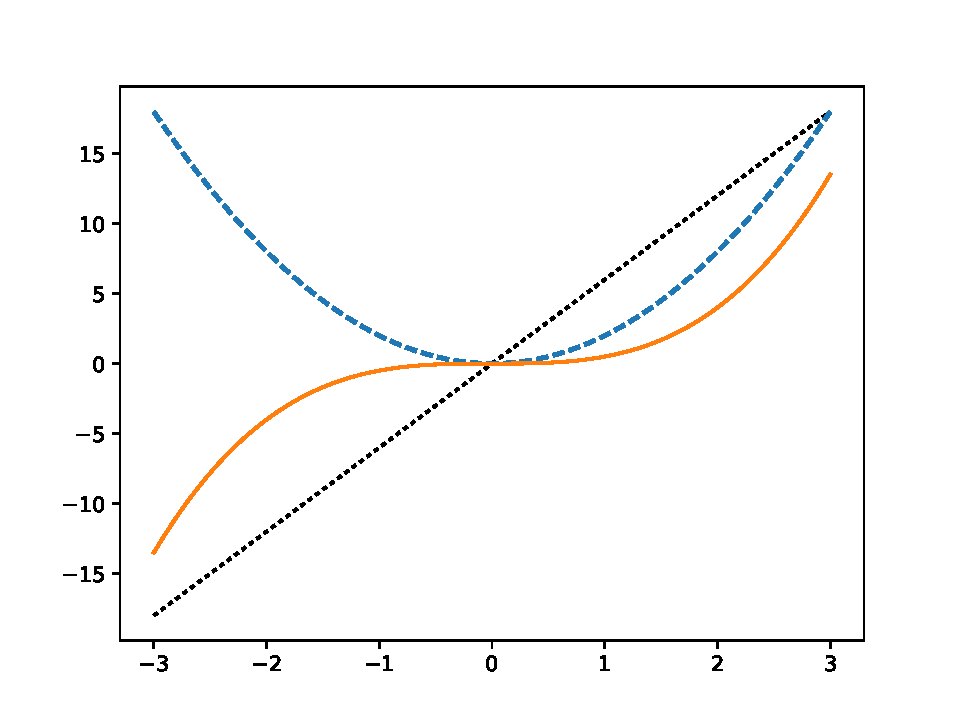
\includegraphics[width=90mm]{plt-plot}
  \caption{Multiline figure}
  \label{fig:plt-plot}
\end{figure}

The command \python{linspace} is used for conveying value to a matrix. Like MATLAB, matrix in \NumPy\ can be regarded as operation unit, such as ``y = 2*x''. Matrix is similar to list or tuple in \Py , but without \NumPy\ you need to type something more complex: ``y = [2*xi for xi in x]'' .

\nextblock You can use \python{plt.hold} to close multiline drawing feature (i.e. figure window can only show you ONE line created by the nearest used \texttt{plot} command).  
\begin{py}
plt.hold(False)
\end{py}

The default setting is blue and solid line. You can simply write like this:
\begin{py}
plt.plot(x, y, 'b-')
\end{py}

\subsection{Line Style, Marker and Line Color}
The line style, marker and line color can be chosen from \autoref{tab:linestylecolor}.

\begin{table}[!hbt]
\centering
\caption{Line style and line color}
\label{tab:linestylecolor}
\begin{tabular}{|*{3}{>{\ttfamily}cl}|}
\hline
\multicolumn{6}{|c|}{Line Styles} \\
'-'	& solid line style &
'--' & dashed line style &
'-.' & dash-dot line style \\
':'	& dotted line style & & & &\\
\hline
\multicolumn{6}{|c|}{Marker Styles} \\
'.'	& point marker &
','	& pixel marker &
'o'	& circle marker \\
'v'	& triangle\_down marker &
'\^{}' & triangle\_up marker &
'<'	& triangle\_left marker \\
'>'	& triangle\_right marker &
's'	& square marker &
'p'	& pentagon marker \\
'*'	& star marker &
'h'	& hexagon1 marker &
'H'	& hexagon2 marker \\
'+'	& plus marker &
'x'	& x marker &
'D'	& diamond marker \\
'd'	& thin\_diamond marker &
'|'	& vline marker &
'\_' & hline marker \\
\hline
\multicolumn{6}{|c|}{Line Colors} \\
`b' & blue &
`g' & green &
`r' & red \\
`c' & cyan &
`m' & magenta &
`y' & yellow \\
`k' & black &
`w' & white & & \\
\hline
\end{tabular}
\end{table}

You can also define color by hex value, or by RGB/RGBA tuple:
\begin{py}
... color='#66ccff' # Uppercase '#66CCFF' also acceptable
... color=(1, 0, 0) # RGB -> Red
... color='0.8' # Gray shade (1.0 is white, 0.0 is black)
\end{py}

As an example, we draw a scatter plot with blue circle (i.e. 'bo' in \mpl):
\begin{py}
x = np.arange(0, 9, 1)
y = x**(1/2)

plt.plot(x, y, 'bo')
plt.show() # `\autoref{fig:plt-plot-2}`
\end{py}

Also you can find command \python{arange}, a command provided by \NumPy\ to create a vector from 0 to 9 (9 is NOT included) with step 1: [0, 1, 2,\ldots ,8]. 

\begin{figure}[!htb]
  \centering
  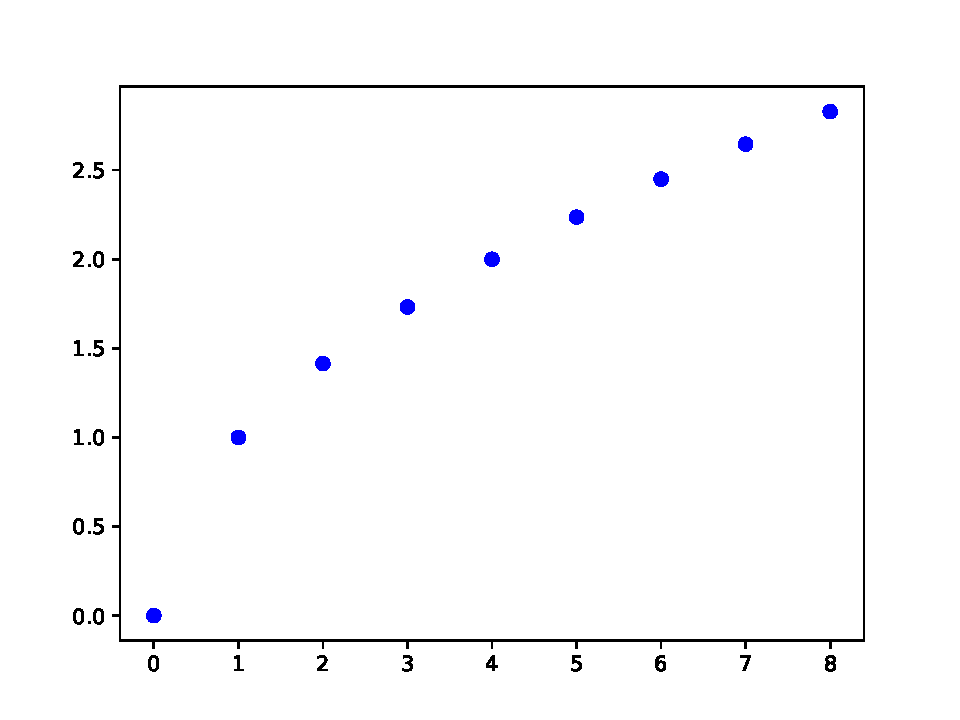
\includegraphics[width=90mm]{plt-plot-2}
  \caption{Scatter figure}
  \label{fig:plt-plot-2}
\end{figure}

Other properties you may use are: \python{markeredgewidth}, \python{markeredgecolor}, \python{markerfacecolor}, \python{markersize}, and:
\begin{py}
# The ratio of ink & space in a dashed line:
linestyle='--', dashes = (3, 1)
# Drawstyle: steps = stair-like
drawstyle = 'default'/'steps'/'steps-pre'/'steps-mid'
# The style of at the end of the line: 
solid_capstyle = 'butt'/'round'/'projecting'
\end{py} 

\section{\texttt{plt.axis/xlim/ylim}}
On most occasions that axis needs setting, those commands will be useful:

\begin{py}
print(plt.axis()) # show current axis
plt.axis([0, 8, 0, 3]) # set current axis
plt.axis(xmin=0, ymax=3) # Only set some specific limits
plt.xlim([0, 8]) # Set X-min and X-max. The same with ylim
\end{py}

Besides, \python{axis} command has some other features:
\begin{py}
# Hide the axis lines and labels:
plt.axis('off')
# equal - Equal scales in X and Y by changing axis limits;
# scaled - Equal scales in X and Y by changing the plot box;
# tight - Change limits to show all data; 
# square - Same Xlim and Ylim range, and same scaling.
plt.axis('equal'/'scaled'/'tight'/'square')
\end{py}

\section{\texttt{plt.figure \& plt.subplot}}
The \texttt{figure}\index{plt!figure} command let you to create many plots in one run. You can have $N$ figure windows if you use \texttt{figure} command for $N$ times. Here's an example:

\begin{py}
x = np.linspace(-3, 3, 100)
y1 = 6*x
y2 = 2*x**2

plt.figure(1) # First figure window
plt.plot(x, y1, 'b-')
plt.figure(2) # Second figure window
plt.plot(x, y2, 'r-')
plt.show()
\end{py}

And \texttt{subplot} allows you to draw many subplot in one figure window\cite{mplwebsite}:
\begin{py}
def f(t):
    return np.exp(-t) * np.cos(2*np.pi*t)

t1 = np.arange(0.0, 5.0, 0.1)
t2 = np.arange(0.0, 5.0, 0.02)

plt.figure(1)
plt.subplot(211)  # Total 2 Row 1 Col. Figure 1 of 2
plt.plot(t1, f(t1), 'bo', t2, f(t2), 'k')

plt.subplot(212, facecolor=(0, 0.2, 0.5))  # Figure 2 of 2
plt.plot(t2, np.cos(2*np.pi*t2), 'r--')
plt.show() # `\autoref{fig:plt-subplot}`
\end{py}

\begin{figure}[!htb]
  \centering
  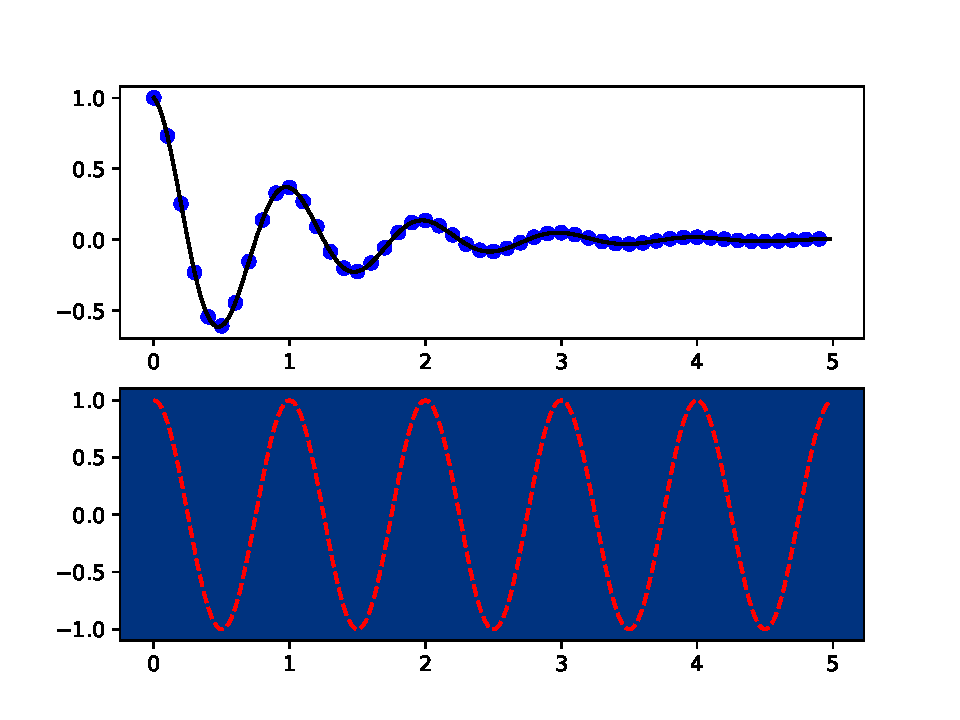
\includegraphics[width=90mm]{plt-subplot}
  \caption{Subplots example}
  \label{fig:plt-subplot}
\end{figure}

\section{\texttt{plt.grid}} 
\begin{py}
x = np.linspace(-3, 3, 100)
y1 = 6*x
y2 = 2*x**2

plt.plot(x, y1, x, y2)
# Simply using "plt.grid(True)" also works
plt.grid(axis='y', linestyle='--', color='0.85')
plt.show() # `\autoref{fig:plt-grid}`
\end{py}

Default value of `\texttt{axis}' is `both'. Value `x' and `y' are also allowed.

\begin{figure}[!htb]
  \centering
  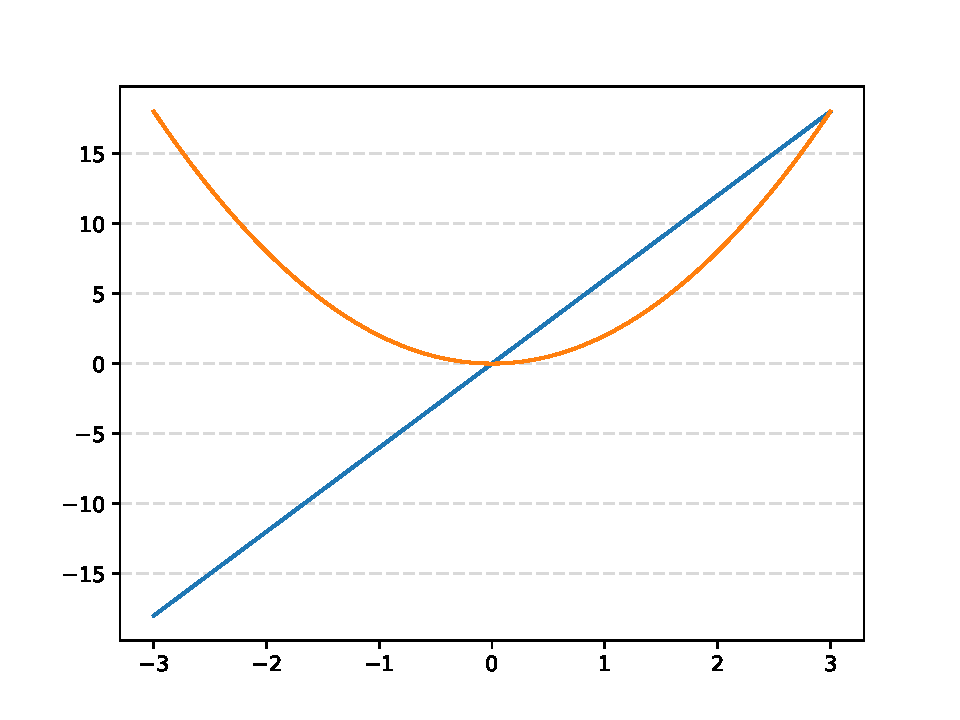
\includegraphics[width=90mm]{plt-grid}
  \caption{Grid example}
  \label{fig:plt-grid}
\end{figure}

\section{\texttt{plt.axis \& plt.xlim/ylim}}
\begin{py}
x = np.linspace(-3, 3, 100)
y1 = 6*x
y2 = 2*x**2

plt.plot(x, y1, x, y2)
plt.axis([-4, 4, -20, 20])
plt.show() # `\autoref{fig:plt-axis}`
\end{py}

\begin{figure}[!htb]
  \centering
  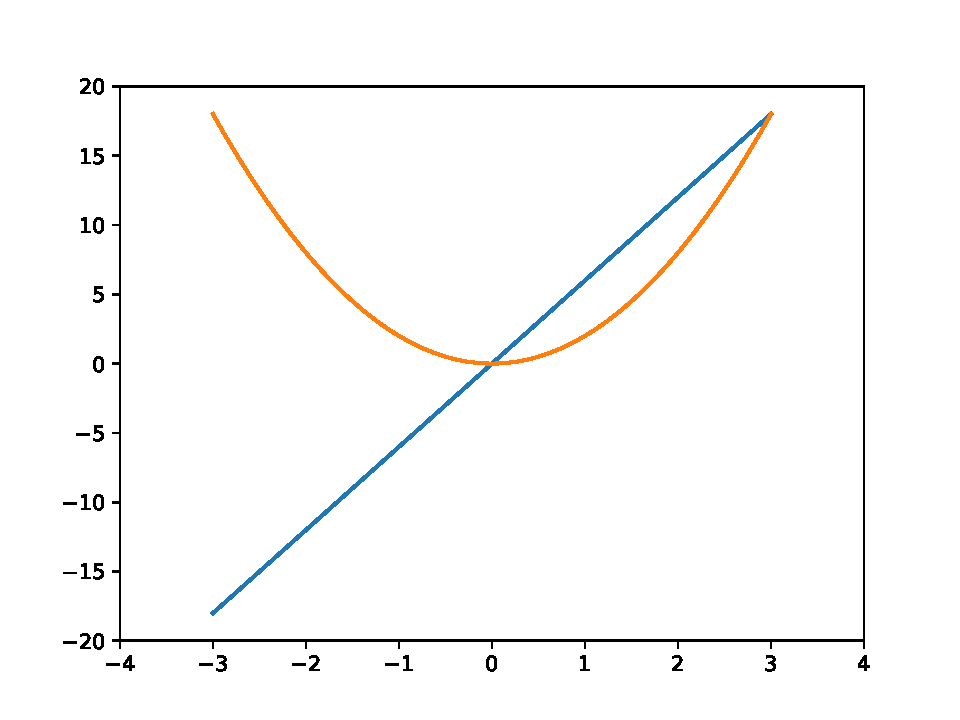
\includegraphics[width=90mm]{plt-axis}
  \caption{Axis setting example}
  \label{fig:plt-axis}
\end{figure}

Line 6 of above is equal to:
\begin{py}
# One para is also allowed if needed: "plt.xlim(xmin=-4)"
plt.xlim([-4, 4]) 
plt.ylim([-20, 20])
\end{py}

\section{\texttt{plt.xticks/yticks}}
\begin{py}
x = np.linspace(-3, 3, 100)
y1 = 6*x
y2 = 2*x**2

plt.plot(x, y1, x, y2)
plt.axis([-4, 4, -20, 20])
plt.xticks(np.linspace(-4, 4, 5))
plt.yticks(np.arange(-20, 20, 10), ['$A$', '$B$', '$C$', '$D$'])
plt.show() # `\autoref{fig:plt-xtick-ytick}`
\end{py}

\begin{figure}[!htb]
  \centering
  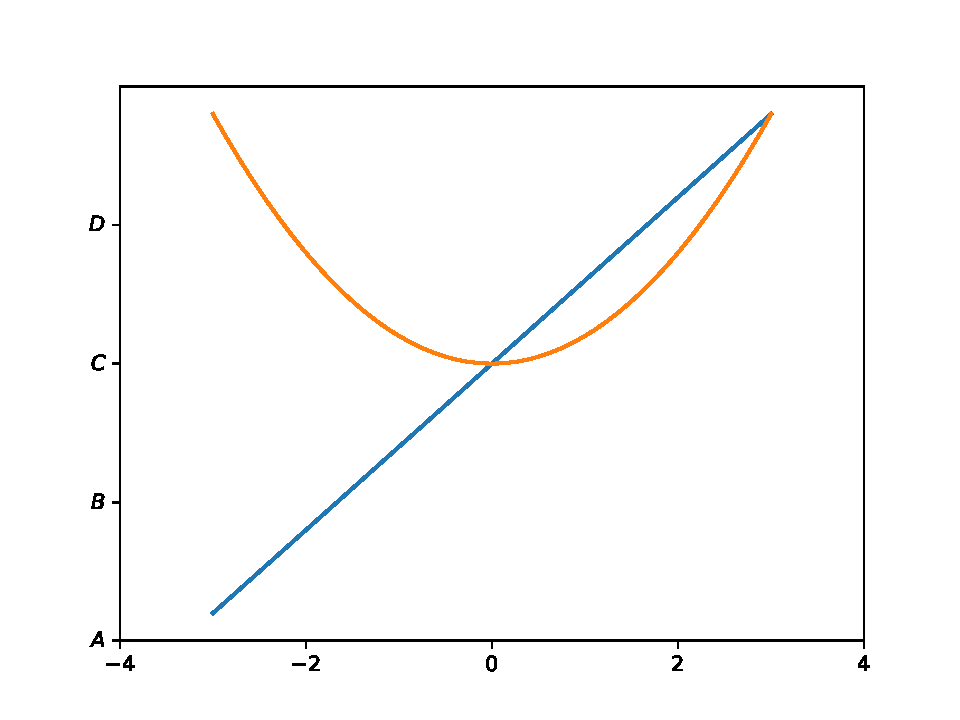
\includegraphics[width=90mm]{plt-xtick-ytick}
  \caption{Change ticks}
  \label{fig:plt-xtick-ytick}
\end{figure}

\begin{py}
# Hide the top and right spine
ax = plt.gca()
ax.spines['right'].set_visible(False)
ax.spines['top'].set_visible(False)
ax.spines['bottom'].set_position(('data', 0))
ax.spines['left'].set_position(('data', 0))
plt.show() # `\autoref{fig:plt-spines}`
\end{py}

\begin{figure}[!htb]
  \centering
  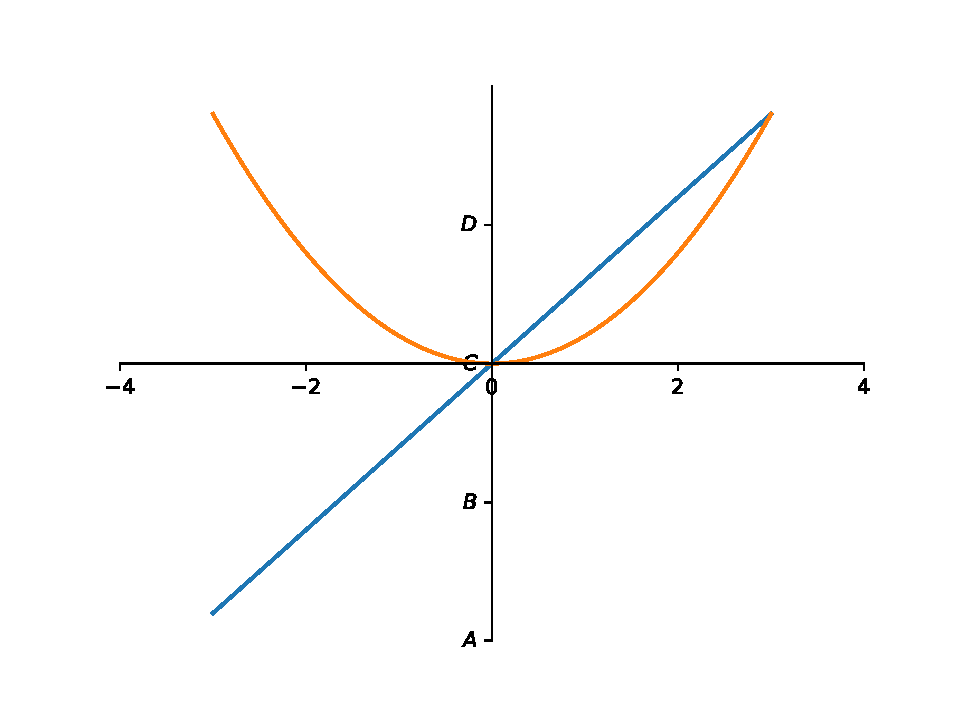
\includegraphics[width=90mm]{plt-spines}
  \caption{Move the axises}
  \label{fig:plt-spines}
\end{figure}

\section{\texttt{plt.title \& plt.xlabel/ylabel}}
\begin{py}
x = np.linspace(-3, 3, 100)
y1 = 6*x
y2 = 2*x**2

plt.plot(x, y1, x, y2)
plt.title('Very simple title here')
plt.xlabel('Times(s)')
plt.ylabel(r'$f(x)=\alpha x^{\beta}$') # LaTeX code included
plt.show() # `\autoref{fig:plt-title}`
\end{py}

\begin{figure}[!htb]
  \centering
  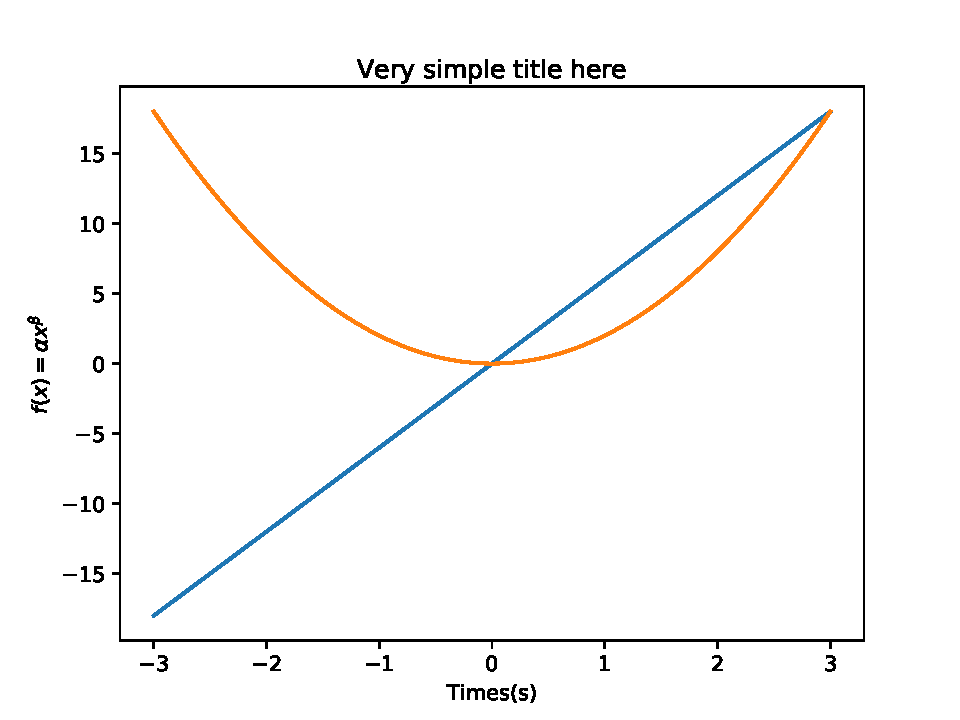
\includegraphics[width=90mm]{plt-title}
  \caption{Title example}
  \label{fig:plt-title}
\end{figure}

\section{\texttt{plt.legend}}
\begin{py}
x = np.linspace(-3, 3, 100)
y1 = 6*x
y2 = 2*x**2

plt.plot(x, y1, label='First')
plt.plot(x, y2, label='Second')
plt.legend(loc='lower center', ncol=2)
plt.show() # `\autoref{fig:plt-legend}`
\end{py}

\begin{figure}[!htb]
  \centering
  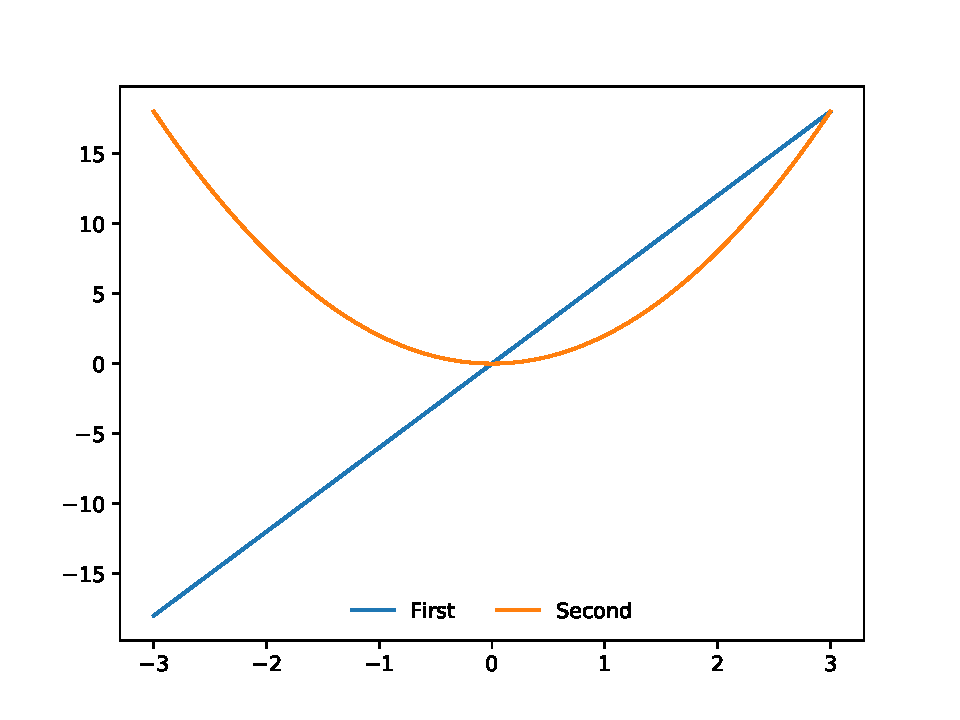
\includegraphics[width=90mm]{plt-legend}
  \caption{Legend example}
  \label{fig:plt-legend}
\end{figure}

\section{\texttt{plt.text}}
\begin{py}
plt.plot([1, 1], [0, 3], color='k', linewidth=0.5, linestyle='--')
plt.text(2, 1, 'Hmm', fontsize=12)
plt.text(1, 1, 'Two lines\n text', horizontalalignment='center')
plt.text(1, 3, 'With box', bbox=dict(facecolor='red', alpha=0.3))
plt.axis([0, 3, 0, 4])
plt.show()  # `\autoref{fig:plt-text}`
\end{py}

\begin{figure}[!htb]
  \centering
  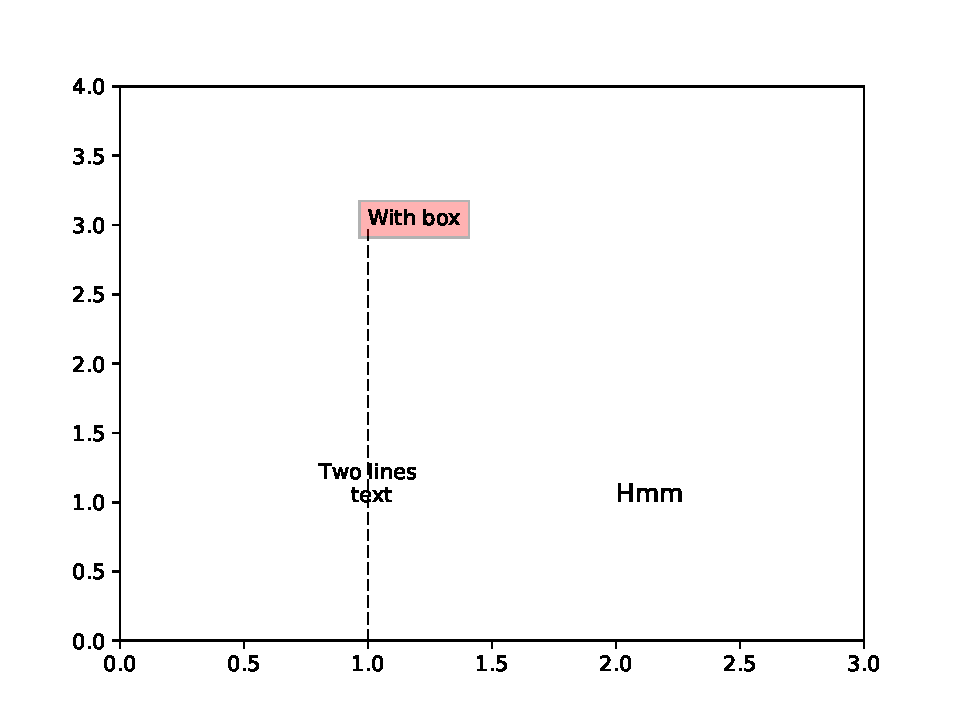
\includegraphics[width=90mm]{plt-text}
  \caption{Text example}
  \label{fig:plt-text}
\end{figure}

%
% Appendix
%

\appendix

\begin{thebibliography}{9}
\bibitem{mplwebsite} Matplotweb Official Website. 
  \newblock \emph{Pyplot Tutorial}, \\ \url{http://matplotlib.org/users/pyplot_tutorial.html}

\bibitem{mplwebsite} Matplotweb Official Website. 
  \newblock \emph{Pyplot API}, \\  
  \url{http://matplotlib.org/api/pyplot_api.html}
  
\bibitem{tosi2009matplotlib} Sandro Tosi.
  \newblock \emph{Matplotlib for Python Developers},
  \newblock Packt Publishing Ltd, 2009
\end{thebibliography}

\end{document}